%
%  problems.tex  2014-01-07  Derrick Kearney
%
%  give specific examples of the kinds of problems we are trying to solve.
%

\chapter{THE HUBCHECK PROBLEM SPACE}
\label{chap:problem}


%\1 Typical problems we see on the hub
%  \2 Website configuration problems
%    \3 User quotas not turned on (0% of 0GB storage meter) hubzero #3750, 3749, 3747, 3746
%    \3 In the My Sessions module, session shortcut and screenshots not turned on, hubzero #3369, 3368, 3367, 3364
%    \3 
%  \2 Hub update problems
%    \3 missing links or expected functionality, hubzero #3642
%    \3 wrong number of tags listed on page, hubzero #3617
%    \3 invalid create dates for groups, hubzero #3552
%    \3 after hub reboot, tools component not turned back on, hubzero #3431
%  \2 Nightly testing problems
%    \3 starting tool session container fails, hubzero #3705
%    \3 starting tool session container fails, connection closed, hubzero #3571
%    \3 accessing tool session container fails, vssh_gateway permission denied, hubzero #3229
%    \3 render server not accessible from tool session container, hubzero #3569
%    \3 submit command fails with exit status 2, missing config files, hubzero #3171
%  \2 Tool Session container upgrades
%    \3 installing submit, pegasus, hubzero #3312, 3308
%    \3 installing rappture
%    \3 /apps directory structure
%\end{outline}


%\1 HUBcheck automates multi-step tasks in the web browser or in the shell
%  \2 HUBcheck web library
%  \2 HUBcheck shell library


%\1 Hub users run into problems while using either the website or the tool session containers.
%  \2 Hub website problems can usually be categorized in three ways:
%     \3 Hub Configuration Issues
%       \4 Module configuration
%       \4 CSS Styling Issues - (HUBcheck does not focus on these types of problems)
%     \3 Hub Upgrade Issues
%     \3 Hub Reboot Issues
%  \2 Hub tool session container problems
%  \2 Hub tasks that require both access to the website and tool session containers.



Problems on the hub creep in without developers noticing. Breakdowns in hub
functionality generally occur when the hub is first set up, after a hub
software upgrade, or after a hub server reboot.  Below, we explore examples of
problems seen on the hub and investigate, at a high level, how HUBcheck can be
used to alert hub developers of the issues.


\section{Hub Configuration Issues}
\label{sec:problem_config}

There are two types of configurations the HUBzero Team seeks to
support: a configuration for hubs managed internally by the group and a
configuration for the open source release of the HUBzero Platform. Out of the
box, the hub provides user friendly default configuration values for the open
source release. Hubs managed internally use a slightly different configuration
because the software often includes advanced features not available in the open
source release, like upgraded middleware and web components. These differences
can lead to misconfigured internally managed hubs. One example where support
for these different configurations can be seen is in the \texttt{My Sessions}
module, available on the user's Dashboard on the hub website.

The \texttt{My Sessions} module was designed to provide a way for users to
manage their active tool session containers. When fully configured, the My
Sessions module can also show a screenshot of the tool session container,
provide a shortcut link to open the tool session container, and display the
user's available disk space on the hub.
\Cref{fig:my_sessions_module_compare} compares a fully configured My Sessions
module, on the left, with one whose features are disabled or not working
properly, on the right.

\begin{figure}[H]
  \centering
  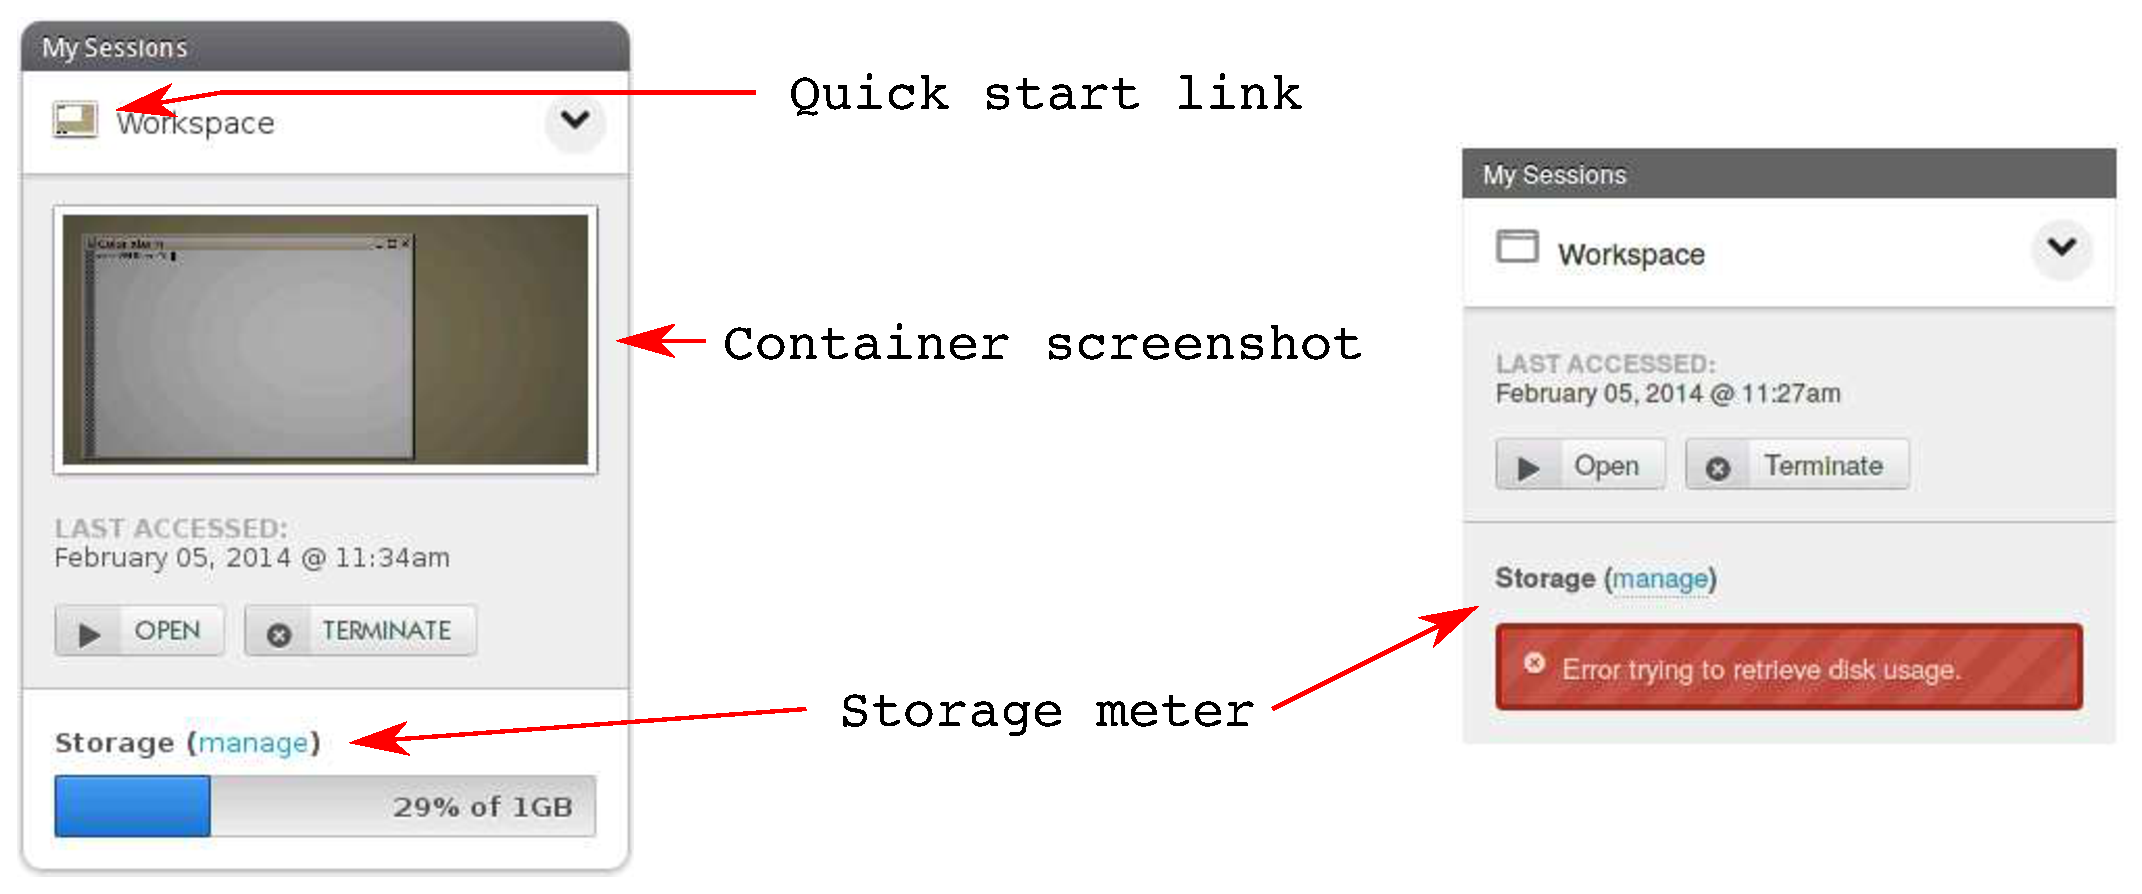
\includegraphics[width=0.98\textwidth]
    {../../images/eps/hub+configuration+dashboard+my+sessions+2.pdf}
  \caption{ The \texttt{My Sessions} module can be configured to show
            screen shots of the tool session containers, provide short
            cut links to access the container, and display the user's
            available disk storage on the hub. The module on the left
            is fully configured showing the container screenshot, an
            enabled quick start link, and storage meter. The module
            on the right has some of these features disabled.}
  \label{fig:my_sessions_module_compare}
\end{figure}


The My Sessions module can be configured to provide the user with a shortcut
link to access active tool session containers and screen shots of applications
running inside of an active tool session container.  Capturing screen shots of
the tool session container is a function performed by the middleware and is not
available in the open source release prior to version 1.2.1. Because of this,
the feature is turned off by default. Hosted hubs, managed by the HUBzero Team,
run an advanced version of the middleware that supports this feature. When new
hosted hubs are launched, turning this feature on is often missed.

Similarly, the availability of the disk usage and quota information depends
upon the hub being configured to show the information and having the
\xfprogramname{telequotad}
% FIXME: should probably cite hubzero-telequotad
service running on the hub's fileserver. When the hub is not configured to show
the disk usage, or the telequotad service is not running, users are shown
messages like those in the image on the right side of
\Cref{fig:my_sessions_module_compare}, explaining that the information is
unavailable or simply stating the used disk space is \textbf{0\% of 0GB} when
the user has no quota set.

When a hub is first installed, there are many settings that can be adjusted to
change the user experience. HUBcheck provides a library to help developers
automate the validation of these settings through the hub's website, from the
user's perspective. Using HUBcheck, developers can write automation scripts
that can login to the hub website as a user, start a tool session container,
and test if the My Sessions module is correctly showing screen shots and
enabling short cut links.


%\begin{enumerate}
%\item login to the hub website as a user
%\item navigate to the user's Dashboard web page
%\item launch a new tool session container
%\item navigate back to the user's Dashboard web page
%\item verify that the new tool session container is
%      listed in the My Sessions module
%\item verify that the tool session container's entry
%      in the My Sessions module contains a shortcut link
%      to open the tool session container.
%\item verify that the tool session container's entry
%      in the My Sessions module contains a screen shot
%      of the tool session container.
%\end{enumerate}


%\begin{figure}[ht!]
%  \centering
%  \includegraphics[width=0.5\textwidth]
%    {../../images/catalyzecare_dashboard_my_sessions_no_screenshot_shortcuts.png}
%  \caption{ The \textit{My Sessions} module on the user's Dashboard shows
%            \textbf{0\% of 0GB} in the storage meter when the user has no
%            quota set. }
%  \label{fig:application_view_working_storage_meter}
%\end{figure}

%These two problems are easy to catch using an automated testing suite
%like HUBcheck. To find them, a HUBcheck test can be written to perform the
%following tasks:

Developers can also write HUBcheck based automation scripts to identify
problems like the improper disk usage calculation mentioned earlier. To do this
by hand a developer would:

\begin{figure}[H]
  \vspace{-10pt}
  \begin{minipage}[c]{0.48\linewidth}
    \begin{enumerate}
    \item login to the hub website as a user;
    \item navigate to the user's Dashboard web page;
    \item locate and read the disk storage string from the web page;
    \item validate the string holds the proper format.
    \end{enumerate}
  \end{minipage}
  \hfill
  \begin{minipage}[c]{0.48\linewidth}
    \centering
    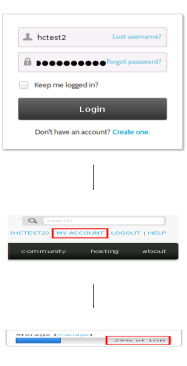
\includegraphics[scale=0.7]
      {../../images/eps/check+user+storage+meter+process+2.pdf}
%    \caption{Process to check that the user's storage meter is being displayed.}
    \caption{Accessing user's storage meter.}
    \label{fig:check_user_storage_meter_process}
  \end{minipage}
\end{figure}


The HUBcheck script shown in
\Cref{lst:dashboard_mysessions_check_storage} follows the same steps.  The
format of the disk storage string should match the format similar to
\textbf{X\% of YGB}, where X is an integer, ranging from 0 to 100, describing
the percentage of the user's available disk that has been used, and Y is a
positive integer describing the amount of disk space available to the user, in
gigabytes.

HUBcheck's web automation library simplifies common tasks like logging into the
hub website and navigating to web pages. The library also provides abstractions
of hub web pages, called page objects, so developers can reuse common blocks of
code and take advantage of a standard library for locating elements on the web
page.


\begin{xcode}{%
  language=Python,%
  label=lst:dashboard_mysessions_check_storage,%
  caption={Checking user's storage meter, using a HUBcheck backed script} %
}
...
# launch the browser and navigate to hub website
hc.browser.get('https://hubzero.org')

# login to the hub website as a user
hc.utils.account.login_as(username,userpass)

# navigate to the user's Dashboard web page
po = hc.catalog.load_pageobject('GenericPage')
po.header.goto_myaccount()

# locate and read the disk storage string from the web page
po = hc.catalog.load_pageobject('MembersDashboardPage')
storage_amount = po.modules.my_sessions.storage.storage_meter()

# validate the string holds the proper format
assert storage_amount != '', 'invalid storage amount returned'
assert storage_amount != '0% of 0GB', 'user quotas not activated'
...
\end{xcode}


\section{Hub Upgrade Issues}
\label{sec:problem_upgrade}

Errors also tend to arise on the hub after software upgrades.  These types of
errors can usually be traced back to configuration changes in upgraded hub
modules, the release of errant software, or pre-existing errors on the upgraded
hub that manifest themselves after the upgrade. Running HUBcheck after a hub
has been upgraded can help identify errors related to hub upgrades before the
user experiences them.

\begin{figure}[ht]
  \centering
  \includegraphics[width=0.5\textwidth]
    {../../images/eps/qahubzero_v1_2_group_create_date_bad_year.pdf}
  \caption{ Sometimes errors show up after a hub upgrade like this one, where
            the create date of a new hub group was not being displayed correctly.
            Finding this type of bug is tedious for a human, but developers
            can use HUBcheck to write tests which verify that multistep processes,
            like creating a group, still produce expected results.}
  \label{fig:group_create_date_bad_year}
\end{figure}


One example of a hub upgrade related error that HUBcheck was able to identify
occurred in the hub's \texttt{Groups} component. The \texttt{Groups} component
allows users to organize content and discussions within the hub community. The
component provides discussion forums, wiki pages, blogs, project spaces and
more. Users can create a group by filling out a web form on the hub website.
Groups on the hub have an overview web page that provides some properties of
the group like group name, description, number of members, join policy and
create date.

In this case, HUBcheck was run on a test hub after a software upgrade. A
failing test alerted developers to an error in displaying the create date for
newly created groups.  With knowledge of the problem, hub developers were able
to identify and fix the the errant code before it was propagated to more
hubs, which would have resulted in additional cleanup work.

To find this type of error, a new group needed to be created on the hub, and
its properties verified. The process of creating and verifying a new group on
the hub can be tedious and error prone for a human, but with HUBcheck it can be
done in a few lines of code in a testing script.


\section{Hub Reboot Issues}
\label{sec:problem_reboot}

When the servers hosting a hub are shut down and brought back up, it is easy
for unexpected problems to arise. From hosts having trouble rebooting to remote
filesystems not being properly mounted over the network, machine reboots are a
time where errors can happen that leave the hub not living up to its fullest
potential.  Developers can exercise hub functions quickly by running HUBcheck
after a reboot. HUBcheck provides the type of automation primitives that
encourage developers to tackle the harder problems to automate, like checking
that render servers are accepting connections from within a tool session
container.

\begin{figure}[]
  \centering
  \includegraphics[width=\textwidth]
    {../../images/hubcheck_block_diagram/tool_session_container_block.pdf}
  \caption{ Simulation tool developers use a tool session container to
            develop and deploy their work on the hub. Checking that the
            containers are properly configured is time consuming for a
            human because of the layers of software between the web
            browser and the container's services like Submit and the
            Visualization servers.}
  \label{fig:tool_session_container_block_diagram}
\end{figure}

One of the key features of a hub is its ability to run interactive simulation
tools that are displayed in the user's web browser. These simulation tools are
run in an environment called a tool session container on an execution host that
is a part of the hub. In their web browser, the user sees a display of the tool
session container that has been projected to them, from the hub, using the VNC
protocol. Hosting the interactive simulation tools on the hub allows the user
to take advantage of many features that would not normally be found on their
own system, like access to grid computing services and powerful rendering
machines for interactive visualization.

The tool session container is a Debian Linux environment that supports the
building of simulation tools by tool content developers and the execution of
tools by hub users. Access to grid computing and render machines are services
provided to the tool session containers. After a reboot of the hub these
services should be restored, and if they are not, the simulation tools may not
work correctly.

There are two ways to access a tool session container. The most frequently used
way is through the web browser. Starting a tool on the hub gets the user access
to a tool session container. This approach doesn't allow the user to automate
interaction in a terminal with a shell. The second way is to connect over SSH,
the secure shell protocol. All tool developers can access a tool session
container in this way. This approach has the advantage that it gives access to
a terminal with a shell, and shell automation tools like Expect
\cite{libes1995exploring} have existed since the mid 1990s.

HUBcheck takes advantage of this second approach to accessing a tool session
container and provides a small, Expect-like, shell automation library. Using
HUBcheck, hub developers can write automation scripts that enter a tool session
container and examine the resources that are supposed to be available for tools
to use, like access to the render servers. They can also write scripts to check
if a render server is accepting connections from within the tool session
container, examine the container firewall setup, installation of software such
as the Rappture Toolkit, access to grid infrastructures through the
use of the \xfprogramname{submit} command, file transfer between the user's desktop
and the user's hub account using the \xfurischeme{sftp}, \xfurischeme{filexfer}, or
\xfurischeme{webDAV} protocols, and simulation tool invocation through
\xfprogramname{invoke\_app}, all under the same conditions a simulation tool would be
making its request from.


\section{Multimodal System Automation}
\label{sec:problem_automation}


HUBcheck's combination of web and shell automation libraries helps it provide
developers with the unique ability to write scripts that capture the user
experience of working in the dual environment system that is the hub. While a
great deal of testing and automation can be performed by libraries that only
access the website, or only access the tool session container, there exists a
set of tasks whose operations span both the website and the tool session
container, that no other single tool can automate. These are the cases of a
growing area of interest within the hub, where information is passed from
resources published on the website to tools running inside of the tool session
container. In hub parlance, this is referred to as \textbf{parameter passing}.

Simulation tools run in a tool session container, either on the same host as
the hub's web server or on a separate execution host. While this approach has
its advantages with respect to deploying tools in a consistent environment --
isolation between different users running tools and isolation between tools and
the web server -- there are also a number of disadvantages, one of which is the
inability to easily pass parameters to the simulation tool before it has
launched.

Launching a simulation tool on the hub involves coordination between both the
hub website and hub middleware. It can be explained in five steps and are shown
in \Cref{fig:start_tool_session_container_diagram}:

\begin{enumerate}
\item User click's link to launch tool from web page.
\item Web link calls PHP function which forwards request to middleware.
\item Middleware starts a new tool session container for the tool.
\item Middleware calls the tool's invoke script inside of the tool session container.
\item Invoke script execs command to start tool's graphical user interface.
\end{enumerate}

\begin{figure}[ht]
  \centering
  \includegraphics[width=\textwidth]
    {../../images/eps/start+tool+session+container+diagram2.pdf}
  \caption{ Simulation tools are started by user's clicking a link on the hub
            website. The link forwards the request to the middleware, which
            handles allocating a tool session container and calling the tool's
            invoke script. The invoke script sets up the environment for the
            tool to run in, and finally, launches the tool.}
  \label{fig:start_tool_session_container_diagram}
\end{figure}

There are a couple of ways to start the process to launch a simulation tool on
the hub. The most obvious way is to use a web browser to navigate to the tool's
\textit{tool information page}, a web page that describes what the tool does,
lists its authors and funding sources, and includes a link to launch the tool.
In the first step, the user navigates to the tool information page and clicks
the link to launch the tool.  Clicking the web link sends a request to the hub
web server asking it to start the tool. The hub web server receives the request
and calls upon the hub middleware to launch the new tool.  In step three, the
middleware supplies a tool session container to run the requested tool.

Tools published on the hub include an \textit{invoke script} which contains all
of the commands necessary to launch the simulation tool, including setting up
system environment variables with prerequisite library and executable paths.
In step four above, the middleware enters the tool session container as the
user, and execs the tool's invoke script to start the graphical user interface.
Lastly, the invoke script sets environment variables for the libraries needed
by the tool and launches the tool.

Version 1.2 of the HUBzero software included new components that allowed users
to interact with learning concepts and data through the use of simulation and
modeling. Two examples of this include the Databases component and the Courses
component. The Databases component allows users to create databases of
information and construct views that help others understand their data. The
Courses component allows teachers to manage an online class, hosted on the hub,
that incorporates hub resources including simulation tools.  With both of these
components, developers may want to pass data that is stored on the hub website
over to a tool running in a tool session container.

To address this need, a new algorithm for allowing parameters to be passed from
the website into a simulation tool running in a tool session container was
created. The algorithm accepts a limited number of data types (file names,
directory names, and integers) and encodes the parameters into the URL used to
launch the tool. The parameters are passed through the hub web server and
middleware, which have the opportunity to check them for validity, and into the
tool session container. Once inside of the tool session container, they are
stored in a file, and the tool developer is responsible for parsing them out of
the file, either through the tool's invoke script, or in the simulation tool
itself.

Whether it is data from a database being fed into a cancer prediction model, or
example parameters for simulating a circuit from a class, passing data between
the website and the tool session container involves many layers of software
that have the opportunity to manipulate or lose the data. Passing data is
difficult to do and tedious to test.  HUBcheck provides the automation
primitives necessary to ease the task of writing scripts that can interact with
the website and tool session container in the same script. In the case of
parameter passing, hub developers were able to use HUBcheck's web and shell
automation libraries to build a test suite to exercise passing parameters to a
simulation tool by crafting both valid and invalid URLs. As a part of the test
suite, numerous simulation tools were installed on the hub and URLs were
generated to match the requirements and restrictions of the parameter passing
algorithm. After launching tools with the specialized URLs, the HUBcheck based
scripts accessed the tool session container running the simulation tool and
verified that the parameters were passed through the tool invocation labyrinth
(which includes the web browser, web server, middleware, and tool session
container), through the tool's invoke script, and to the tool where they could
be processed.

